\documentclass{article}
\usepackage[utf8]{inputenc}
\usepackage{amsmath}
\DeclareMathOperator*{\argmax}{\arg\!\max}
\usepackage{booktabs}
\usepackage{geometry}
\usepackage{graphicx}
\geometry{a4paper,left=2cm,right=2cm}
\usepackage{subfigure}
\usepackage{parskip}
\usepackage{float}

\title{Looking for Controversy\\ {\large an ensemble approach to confidence rated prediction} }
\author{}
\date{November 2022}

\begin{document}

\maketitle

\section{Introduction}

Distinguishing between easy and hard examples is an active area of
research~\cite{}. Most of this research is based on quantifying the
hardness of an example by considering the number of learning
iterations required to get the correct label on same example. This
requires knowing the correct label and is therefor hard to apply to
unlabeled test examples.


Modern DNN have increasingly complex architectures involving tens of millions of parameters. Experience shows that increasing the depth and width of the DNN generally leads to better performance. The question we ask is whether increasing the number of parameters is equally important for every test example. We carried some experiments using CIFAR-10. Not surprisingly, we find that different examples require different levels of complexity. 

What {\em is} surprising, however, is the fact that for {\em most} examples a very simple network suffices, only a small fraction of the examples benefits from complex networks. We call examples of the first type {\em easy} and those of the second type {\em hard}. our results suggest that the hardness of an example is an {\em inherent} property of the example and depends only weakly on the type and architecture of the network.

Prior work on this subject~\cite{} is based on the amount of training required to get the example labeled correctly. The problem with this measure is that it requires knowing the correct label and therefor cannot be used at test time. We suggest an ensemble-based approach to measure hardness that does not require knowing the true label.





\section{Related Work}
\cite{stacked_ovr}introduced a framework to deal with multiclass classification task in a one-vs-rest(OVR) way, which is similar to ours that treat each 10-class classification task as 10 binary classification tasks. It also trains multiple classifiers. However, its classifiers are not independent and they work in a stacked order and each classifier is responsible for one class. This paper also pay attention to easy classes and confusing classes and it uses the classes’ easiness to arrange the order of the classifiers.
The key differences to our work are(Need further verify, I haven’t carefully read the details yet): (1)It need labels to define the confusing classes. (2)Whether an example is confusing only matters in the training stage, it no longer cares if it’s confusing in the inferencing stage.

\cite{deephash} focus on building hash for images to make search and retrieve of the images efficient. And it pay attention to the easy and hard examples. However, it needs labels to tell which one is easy or hard. And it only focus on the easiness on training process.

\cite{focal_loss} This paper mentioned a concept: Focal Loss(Not originated in this paper). It also focus on the uncertainty of the classifier’s prediction. But simply using the difference between the predicted score and ground truth as the measure of uncertainty which is very different from ours.

I will look for more paper focusing on easy-confusing examples. Till now, I find most works that pay attention to the easiness and confusion of examples are only trying to make use of it in the training stage to improve the training process. After they get the trained framework, they no longer care about whether an example is easy or confusing on the inference stage, but to simply predict a label in the classical way. But our framework can distinguishing the hardness of the examples on the inference stage, and is able to tell the uncertainty quantitatively.

\section{Theory}

Many learning algorithms are based on finding the single best
rule. Ensemble methods such as Bagging and Random Forests are based on
combining many rules, each of which is close to
otimal. Averaging/voting across the rules results in a more stable and
more accurate rule.  We use a similar logic for classsification with
one important twist: when the ratio between +1 and -1 predictions is
close to 50\%/50\% our combination rule outputs 0, which can be
interpreted as ``I don't know'' (IDK).

Figure~\ref{fig:duality} depics the behaviour of an ensemble of classifiers
in the dual spaces: the sample space and the classifier space.

\begin{figure}[H]
    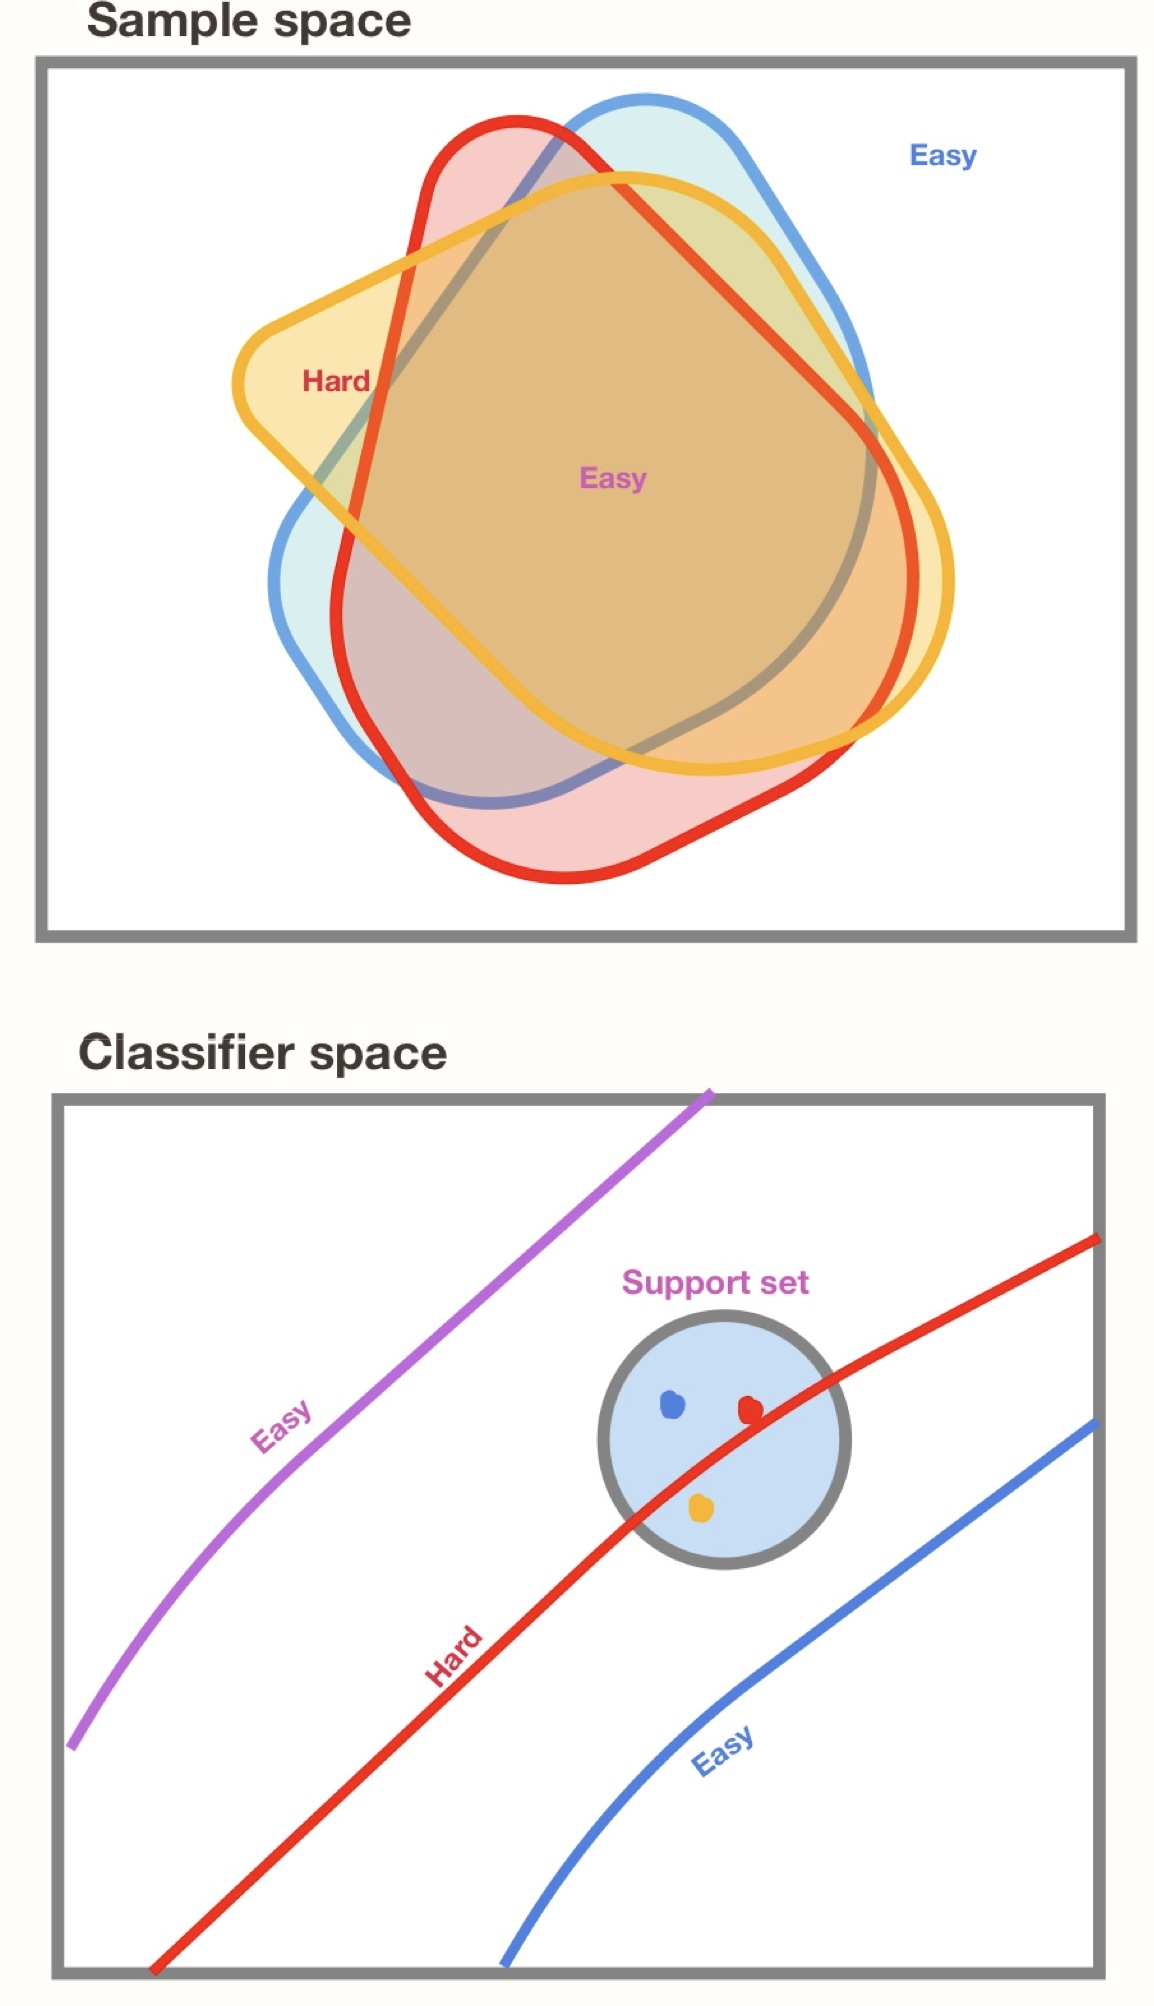
\includegraphics[width=\textwidth]{figs/SupportSet.jpg}
\label{fig:struc}
\caption{\textbf{Duality between classifiers and examples} Each point
  in the sample space figure corresponds to a sample, the three shaded
  sets correspponds to an ensemble of 3 classification rules with
  similar training error. ``Easy -'' is an instance on which the
  ensemble predicts unanimously ``-'', while ``Easy+'' is an instance
  on which the unanimous prediction is ``+''. It is this unanimity
  that makes the instance ``easy''. The hard instance is one on which
  classifiers disagree.  The classifier space (parameter space),
  demonstrates the same relationships between instances and
  classifiers, but here each classifier is a point and the instances
  define boundaries between classifiers that predict ``+' or ``-'' on
  the instance. THe {\em support set} is the set of classifiers whose
  performance is close to optimal. The three dots correspond to the
  ensemble of three classifiers. Finally, easy instances are ones on
  which the rules in the support set are unanimous, while the hard
  example splits the support set in two. \label{fig:duality}}
\end{figure}


\subsection{Binary Case}
In a normal binary classification task, given an input $\textbf{x}$, the predictor will output either $+1$ or $-1$. Our framework not only predicts whether the example is negtive or positive, but also estimates the confidence of the prediction. And when the confidence level is not high enough, we output $0$ rather than $+1$ or $-1$ for "I don't know". 

Usually in a binary classification task, a neural networks predictor calculates a real value. In the training stage this value can be further transfered by a sigmoid funtion to a real value ranging from 0 to 1 and then pluged into the loss function; while in the inferencing stage, this value can be compared with 0 to decide whether this example belongs to the positive class or the negative class. Denote this value calculated by predictor $f \left(\cdot , \mathcal{P}\right)$ as $O_f \left(\cdot , \mathcal{P}\right)$. If $O_f \left(x , \mathcal{P}\right)$ is larger than 0, the example will be classified into the positive class, otherwise the negative class.

\textit{\textbf{Assumption}} As we change the pertubation $\mathcal{P}$ to get $O_f \left(x , \mathcal{P}_1\right), O_f \left(x , \mathcal{P}_2\right),\cdots, O_f \left(x , \mathcal{P}_i\right),\cdots,O_f \left(x , \mathcal{P}_E\right) $, the values $O_f \left(x , \mathcal{P}_i\right)$ obeys a normal distribution $\mathcal{N}(\mu,{\sigma}^2)$. 

The mean value $\mu$ should be positive if this example belongs to the positive class and negative if it belongs to the negative class. After training an ensemble $f \left(\cdot , \mathcal{P}_1\right), f \left(\cdot , \mathcal{P}_2\right),\cdots, f \left(\cdot , \mathcal{P}_i\right),\cdots,f \left(\cdot , \mathcal{P}_E\right) $, we can esitimate how confident we are to say $\mu$ is positive or negative based on $O_f \left(x , \mathcal{P}_1\right), O_f \left(x , \mathcal{P}_2\right),\cdots, O_f \left(x , \mathcal{P}_i\right),\cdots,O_f \left(x , \mathcal{P}_E\right) $. This can be done by \textit{t-test}. The null hypothesis is $\mu = 0$, and the \textit{t}-statistic is: 

\begin{equation}
    t = \frac{\overline{O}_f\left(x , \mathcal{P}\right)}{S/\sqrt{E}}
\end{equation}

where
    \begin{eqnarray}
            \overline{O}_f\left(x , \mathcal{P}\right) &= \frac{1}{E} \sum_{i=1}^E O_f\left(x , \mathcal{P}_i\right) \\
            S^2 &= \frac{1}{E-1} \sum_{i=1}^E {(O_f\left(x , \mathcal{P}_i\right) - \overline{O}_f\left(x , \mathcal{P}\right))}^2
    \end{eqnarray}

denote the $\textit{p}$-value of the test as $\textit{p}$, we define our confidence as:
\begin{equation}
    confidence = -sign( \overline{O}_f\left(x , \mathcal{P}\right))*log(\textit{p})
\end{equation}

If the predictors are very confident that the example belongs to the positive class, the confidence should be a very large positive value; if the predictors are confident of the negtatice class, it should be a very small negative value. If the predictors are unsure, the confidence value would be close to 0. We can set a threshold to discriminate class+ and class-. Further, with this confidence value, we can set one threshold for confidence class+ and another thereshold for confident class-. In the regime between the two thresholds, the predictors will say "I don't know".

\subsection{Multiclass Case}\label{sec:multi}
In a multiclass classification task, $ \textbf{O}_f \left(x , \mathcal{P}\right)$ is no longer a real value but a $R^C$ vector, $C$ is the number of classes. In the training stage, a softmax can be operated on $ \textbf{O}_f $ and further used in the loss function. In the inferencing stage, $\max_{j} \textbf{O}_{f,i}$ will be taken as the final prediction result, where $\textbf{O}_{f,j}$ refers to the $j$th dimension of the $ \textbf{O}_f $ vector.

To apply our \textit{t-test}-based method, we take each multiclass classification task as multiple binary classification tasks. Based on $\textbf{O}_{f,j} \left(x , \mathcal{P}_1\right),\cdots, \textbf{O}_{f,j} \left(x , \mathcal{P}_i\right),\cdots,\textbf{O}_{f,j} \left(x , \mathcal{P}_E\right) $, we can calculate the \textit{t}-statistic $\textit{t}_j$ and get the \textit{p}-value $\textit{p}_j$ and finally the confidence value $\textit{confidence}_j$ for class $j$. 

We can have different ways to make use of the confidence values, for example:
\begin{enumerate}
    \item The class with the largest confident value will be the predicted class.
    \item Instead of predicting one class, the class with the largest confident value and classes whose confidence is no smaller than the largest by a certain amount will form a prediction set.
    \item We can set a threshold as in the binary case. If $\textit{confidence}_j$ is smaller than the threshold, then the example doesn't belong to class j, otherwise the predictors think the example belongs to class j. Similarly, we can set two thresholds for confident of class j, confident not class j and "I don't know".
\end{enumerate}

The second and the third ways bring a problem: the example may belong to multiple classes or none of the classes. When this happens, it suggests that this example is a "hard" example, because it makes the predictors confused among these classes. The experiment section shows that this confusion indeed happens for human. Therefore, it can be benifit to allow the predictors to say that they are confused and further careful actions are needed to make a decision(For example, call stronger predictors to classify the example), rather than simply give a prediction without confidence. 


Let $\mathcal{D}$ be a dataset containing $\left\{\left( \textbf{x}_i ,y_i\right)\right\}_{i=1}^N $,where $\textbf{x}$ is the oberserved feature vector, $y$ is the label in a classification task or a numerical value in a regression task. For a predictor with a specific architecture $f$ (For example, a ResNet),we can apply a pertubation $\mathcal{P}$ in the training process of $f$ and get a predictor $f \left(\cdot , \mathcal{P}\right)$. When a new observed feature vector $textbf{x}$ comes, the predictor gives a prediction $f \left(\textbf{x} , \mathcal{P}\right)$. Since there are many different kinds of predictors, we can also train a set of predictors with different architectures $f_1,f_2,\cdots,f_i,\cdots,f_K$

\begin{figure}[H]
    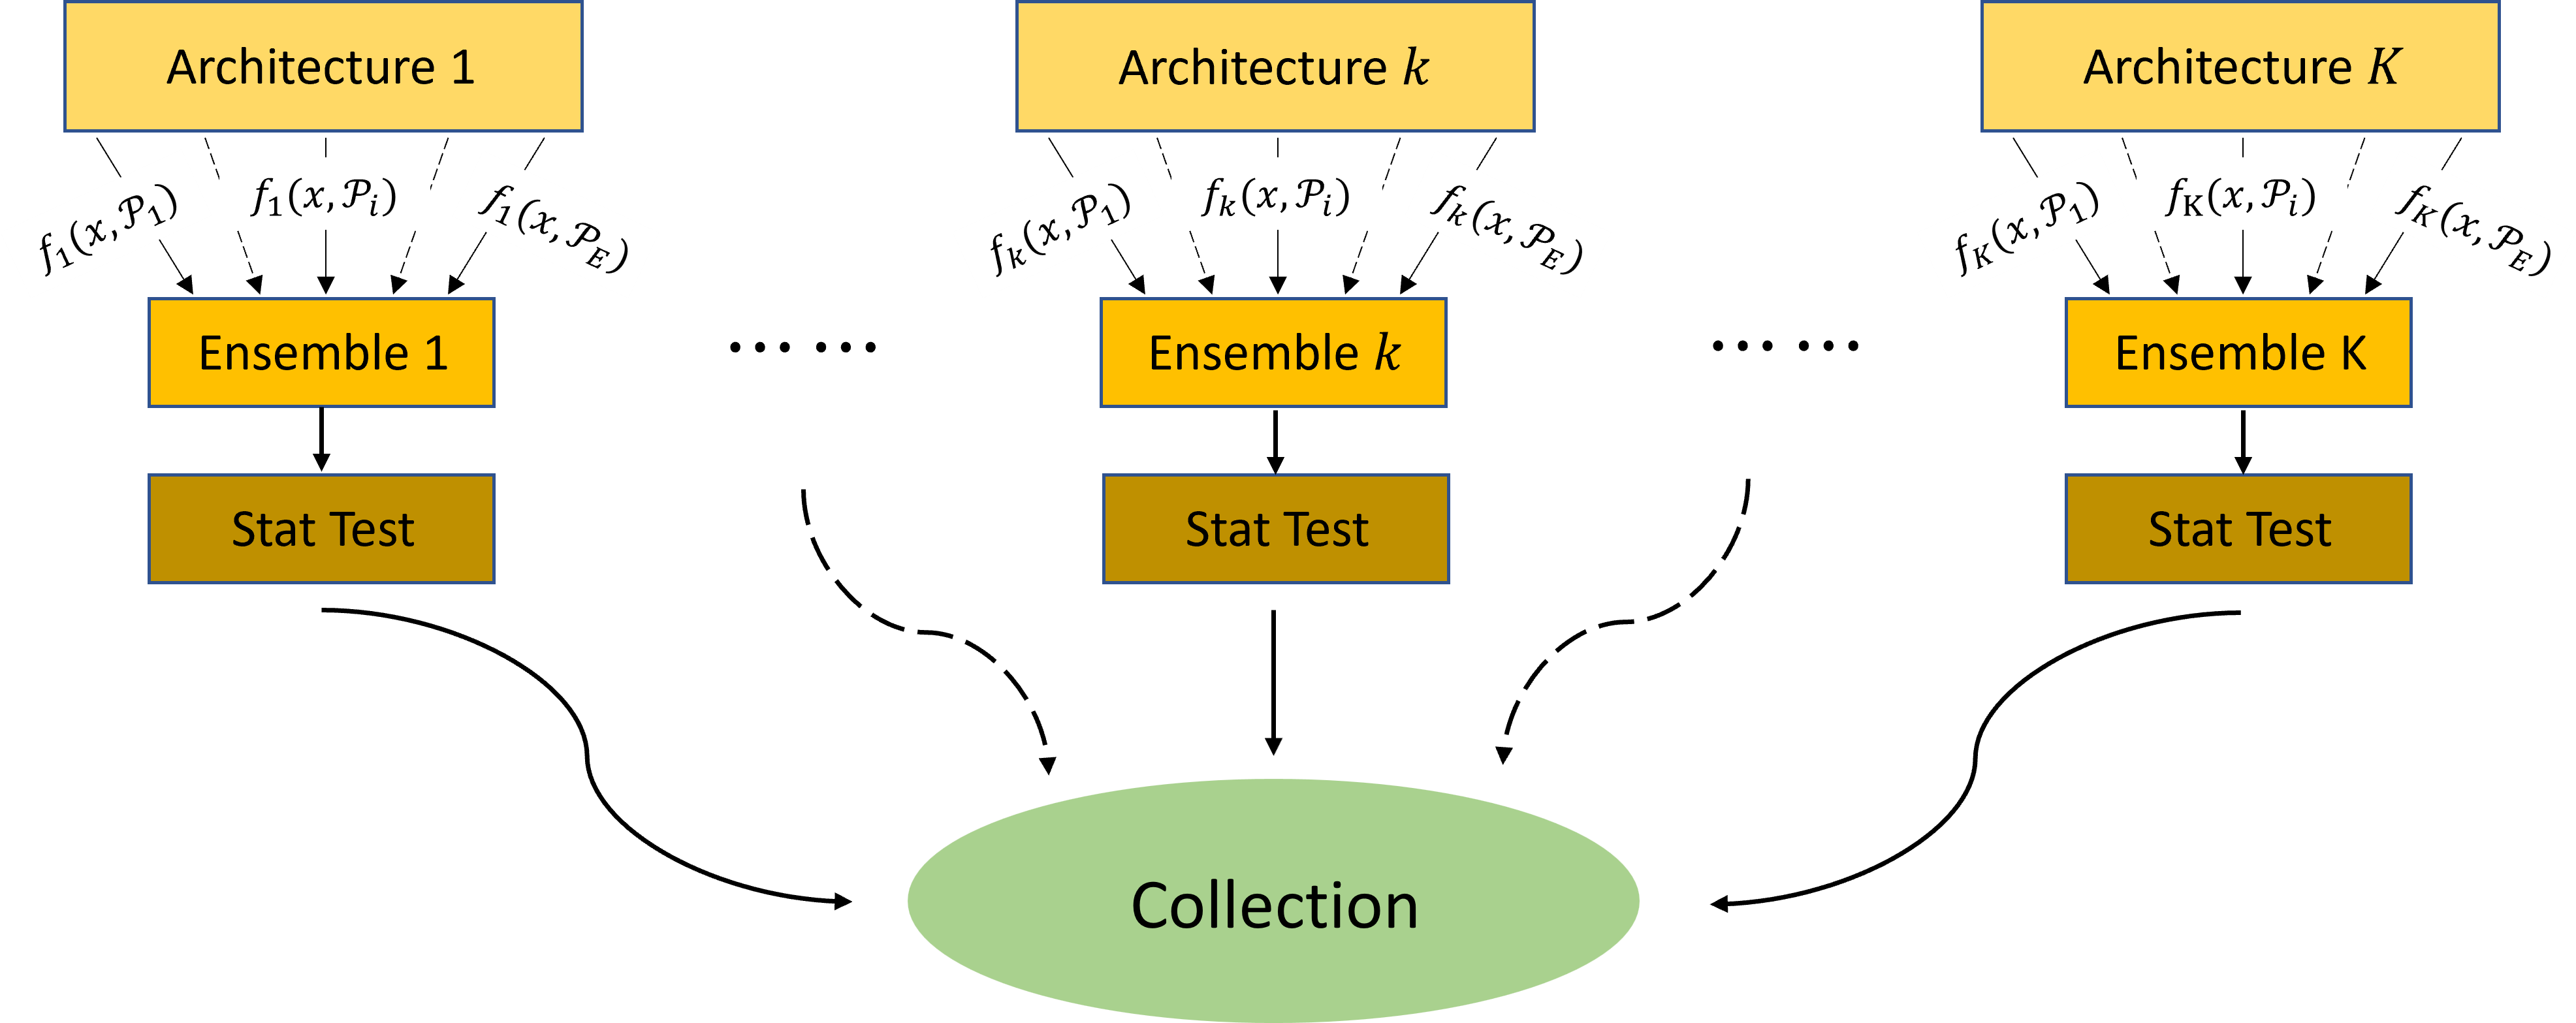
\includegraphics[width=\textwidth]{figs/overall_structure.png}
\label{fig:struc}
\caption{\textbf{Structure of Our Framework}}
\end{figure}

\subsection{Three types of Pertubations: BootStrap, Architecture Starting Points and Architecture }
There are two common ways to pertubate the training process:

\textit{\textbf{Bootstrap}} We can construct a training set $\mathcal{T}$ by randomly draw $M$ examples $\left\{\left( \textbf{x}_i ,y_i\right)\right\}_{i=1}^M $ from $\mathcal{D}$ with replacement. We can sample a set a $\mathcal{T}_1,\mathcal{T}_2,\cdots,\mathcal{T}_i,\cdots,\mathcal{T}_E$ independently, and train a $f$ on each of the training set.
This will generate a set of predictors $f \left(\cdot , \mathcal{T}_1\right), f \left(\cdot , \mathcal{T}_2\right),\cdots, f \left(\cdot , \mathcal{T}_i\right),\cdots,f \left(\cdot , \mathcal{T}_E\right) $ with the same architecture but different parameters.

\textit{\textbf{Random Starting Point}} We take the entire dataset $\mathcal{D}$ as the training set, yet change the initialization of the paremeters in the architecture $f$(For example, use different random seeds to initialize the neural networks). With different starting points $\mathcal{S}_1,\mathcal{S}_2,\cdots,\mathcal{S}_i,\cdots,\mathcal{S}_E$ of the parameters, we can train a set of predictors $f \left(\cdot , \mathcal{S}_1\right), f \left(\cdot , \mathcal{S}_2\right),\cdots, f \left(\cdot , \mathcal{S}_i\right),\cdots,f \left(\cdot , \mathcal{S}_E\right) $



\subsection{Why Ensemble Works}
This section is the analysis of why the aggregation of the ensemble works better than a single predictor.
\subsubsection{For Regression Tasks}
In regression, a common aggregation method is to calculate the average of the ensemble outputs known as \textit{Bagging}, which is:

\begin{equation}
    f^A\left(x\right) = \frac{1}{E}\sum_{i=1}^{E} f\left(x,\mathcal{P}_i\right)
\end{equation}

as $E\rightarrow\infty$, we have:
\begin{equation}
    f^{A*}\left(x\right) = \mathcal{E}_\mathcal{P}\left[f\left(x,\mathcal{P}\right)\right]
\end{equation}

The expectation of the squared error for a single model is:
\begin{eqnarray}
    \mathcal{E}_\mathcal{P}\left[{\left(y-f \left(\textbf{x} , \mathcal{P}\right)\right)}^2\right] &= y^2 - 2y\mathcal{E}_\mathcal{P}\left[f\left(x,\mathcal{P}\right)\right] + \mathcal{E}_\mathcal{P}\left[f^2\left(x,\mathcal{P}\right)\right] \\
    &= y^2 - 2y\mathcal{E}_\mathcal{P}\left[f\left(x,\mathcal{P}\right)\right] + \mathcal{E}^2_\mathcal{P}\left[f\left(x,\mathcal{P}\right)\right]+\mathcal{E}_\mathcal{P}\left[f^2\left(x,\mathcal{P}\right)\right]-\mathcal{E}^2_\mathcal{P}\left[f\left(x,\mathcal{P}\right)\right] \\
    &= {\left(y-\mathcal{E}_\mathcal{P}\left[f\left(x,\mathcal{P}\right)\right]\right)}^2+\mathcal{E}_\mathcal{P}\left[f^2\left(x,\mathcal{P}\right)\right]-\mathcal{E}^2_\mathcal{P}\left[f\left(x,\mathcal{P}\right)\right] \\
    &= {\left(y-f^{A*}\left(x\right)\right)}^2 + Var\left(f\left(x,\mathcal{P}\right)\right)
\label{equ1}
\end{eqnarray}

The equation \ref{equ1} shows that the expectation of the squared error for a single predictor is larger than the squared error of the aggregation. And the difference is just the variance of the predictor outputs over the pertubation.

\subsubsection{For Classification Tasks}
Assume we have $C$ classes in a classification task, for a given $\textbf{x}$, use $P(j|\textbf{x})$ to denote the "Ground Truth" probability that $\textbf{x}$ belongs to class $j$, we will further discuss what the "Ground Truth" means in later section, here let's just simply take it as the true probability.
Given an input $\textbf{x}$, a single predictor will give a prediction among classes ${1,2,\cdots,j,\cdots,C}$. With an ensemble, we can measure how often the predictors will give the predictions, which is:
\begin{equation}
    Q(j|\textbf{x}) = \frac{1}{E}\sum_{i=1}^{E}I(f(\textbf{x},\mathcal{P}_i)==j)
\end{equation}
where $I(\cdot)$ is the indicator function. Again, as $E\rightarrow\infty$, we have:
\begin{equation}
    Q^*(j|\textbf{x}) = \mathcal{E}_\mathcal{P}[I(f(\textbf{x},\mathcal{P})==j)]
\end{equation}

A common method to make use of the ensemble know as \textit{Majority Vote} is picking $\argmax_{1\leq j\leq C} Q^*(j|\textbf{x})$ as the final classification output. 

The expectation of a single predictor being correct is:
\begin{equation}
    \sum_{j=1}^{C}Q^*(j|\textbf{x})P(j|\textbf{x})
\end{equation}

However, as \cite{Bagging} indicates, if the ensemble of predictors is order-correct, which means:
\begin{equation}
    \argmax_{1\leq j\leq C} Q^*(j|\textbf{x}) = \argmax_{1\leq j\leq C} P(j|\textbf{x})
\end{equation}
Not necessarily to be accurate, the ensemble's expectation of being correct is $\max_{1\leq j\leq C} P(j|\textbf{x})$, which is no worse than a single predictor.  \cite{Bagging} gives an example where $P(1|\textbf{x})=0.9$, $P(2|\textbf{x})=0.1$ and $Q*(1|\textbf{x})=0.6$, $Q*(2|\textbf{x})=0.4$. The expectation of a single predictor being correct is $0.58$, but for the ensemble, it's $0.9$

\subsection{More on the Classification task}
In the above section, we know that being order-correct is important for a classification task when making using of an ensemble. Clearly it's not realistic to train infinite predictors to get $Q^*$. If the ensemble size is not large enough, simply applying the majority vote may not give reliable prediction.

\section{Method}

\section{Experiment Result}
This section shows the experiment results on \textit{CIFAR10}\cite{cifar10} and \textit{CIFAR10H}\cite{cifar10h}. \textit{CIFAR10} includes 50000 image-label pairs for training and 10000 image-label pairs for testing. \textit{CIFAR10H} includes extra information for each image which is the frequencies of each label to be chosen as the true label by a group of human labeler. The architectures we used include: ShuffleNet, ShuffleNetV2, MobileNetV2, Regnetx, MobileNet, Efficientnetb0, GoogleNet, Densenet121, Resnext29, ResNet18, SeNet18, SimpleDLA, VGG19, DPN92(Will add citition for these architectures). Table\cite{table:arc_basic} shows the basic information of these architectures.

\begin{table}[H]
\centering
\begin{tabular}{llrrrrr}
    \toprule
    {} &  Parameter & \multicolumn{3}{l}{Forward Time(ms)} & \multicolumn{2}{l}{Single Predictor Accuracy} \\
    {} &      Numbers &  RTX 3080Ti & RTX 3060 &     CPU &  Bootstrap & Random Start \\
    \midrule
    shufflenet     &     925,618 &       2.016 &    7.815 &  13.995 &    0.88802 &     0.895520 \\
    shufflenetv2   &   1,263,854 &       1.867 &    7.341 &   5.931 &    0.88535 &     0.890430 \\
    mobilenetv2    &   2,296,922 &       1.717 &    6.694 &   7.592 &    0.89370 &     0.889671 \\
    regnetx        &   2,321,946 &       2.115 &    7.400 &   8.260 &    0.93330 &     0.938220 \\
    mobilenet      &   3,217,226 &       0.777 &    2.981 &   3.424 &    0.87632 &     0.873603 \\
    efficientnetb0 &   3,599,686 &       2.474 &   10.068 &  10.929 &    0.88585 &     0.896610 \\
    googlenet      &   6,166,250 &       2.990 &   10.722 &  30.060 &    0.93784 &     0.947831 \\
    densenet121    &   6,956,298 &       4.905 &   18.762 &  22.279 &    0.93735 &     0.945434 \\
    resnext29      &   9,128,778 &       1.335 &    4.723 &  24.190 &    0.93952 &     0.948639 \\
    resnet18       &  11,173,962 &       0.930 &    3.375 &   7.130 &    0.93688 &     0.948173 \\
    senet18        &  11,260,354 &       1.417 &    5.282 &   8.088 &    0.93591 &     0.945290 \\
    simpledla      &  15,142,970 &       1.769 &    6.415 &  12.596 &    0.93045 &     0.943860 \\
    vgg19          &  20,040,522 &       0.855 &    3.154 &   6.660 &    0.91733 &     0.931955 \\
    dpn92          &  34,236,634 &       4.712 &   17.596 &  58.489 &    0.94122 &     0.948508 \\
    \bottomrule
\end{tabular}
\caption{\textbf{Basic Properties of the Architectures}: Parameter numbers refers to the number of trainable parameters in each architecture. Forward Time refers to the averaged forward propagation time for one CIFAR image. We tested these values on 3 different devices: Nvidia RTX 3080Ti, Nvidia RTX 3060 and 11th Gen Intel(R) Core(TM) i5-11400F CPU.The last two columns show the accuracy of single predictors trained with different pertubation methods. Bootstrap samples 30000 examples from the 50000 training data.}
\label{table:arc_basic}
\end{table}

\subsection{Compare the Strong and Weak Architectures}
As explained in section \ref{sec:multi}, each multiclass example can be transformed to multiple binary case. In our settings, each image can be divided to 10 image-class pairs. Each pair will have a label $+$ if the image belongs to this class, or $-$ if it doesn't.To compare the difference of the confidence values by weak and strong architectures, we assign a $\left[S,W\right]$ coordinates for each image-class pair. The $S$ value represents the confidence value for a strong architecture, while the $W$ represents a week. In this way, the 10000 test examples will be 100000 points on the $S-W$ plane. Figure \ref{fig:kde_vgg_mobilenet} shows the density distribution of these points with KDE plots.
\begin{figure}[H]
    \centering
    \subfigure[Human: Cat(1.0); Machine: Dog]{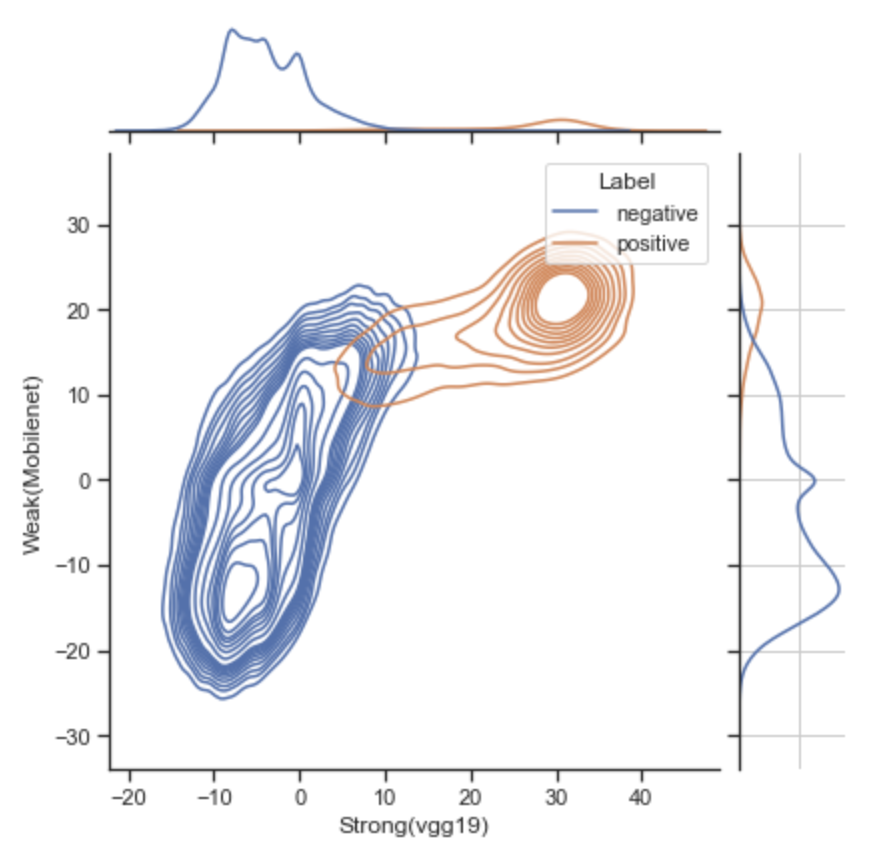
\includegraphics[width=2.5in]{figs/mobilenet_vgg_kde10_bs.png}}
    \subfigure[Human: Cat(1.0); Machine: Dog]{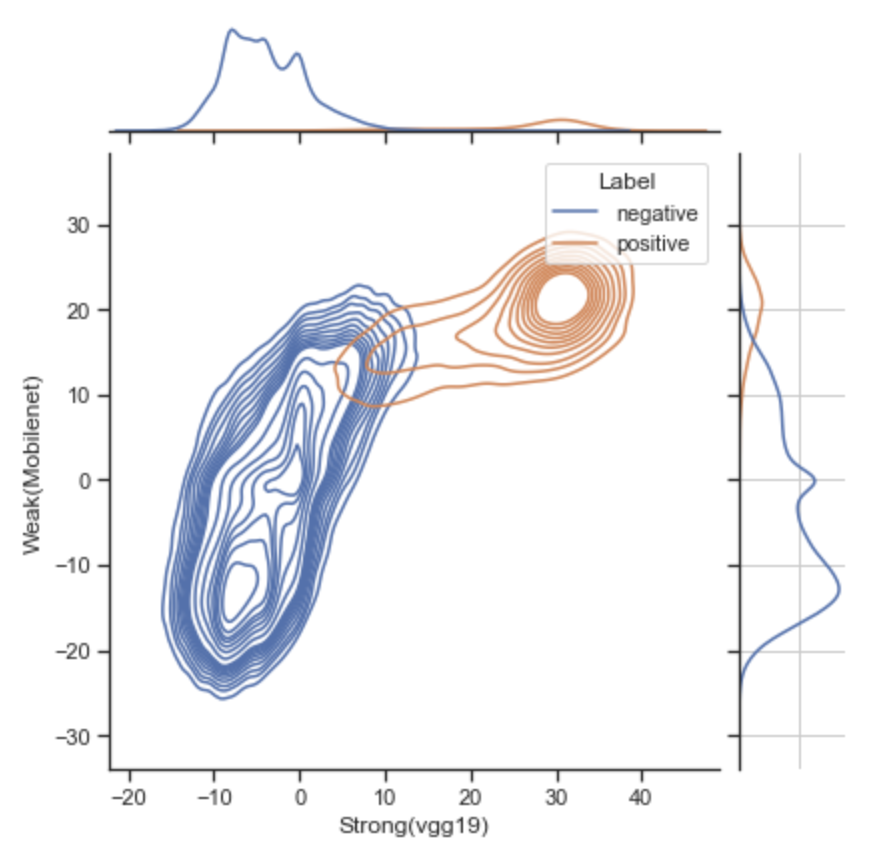
\includegraphics[width=2.5in]{figs/mobilenet_vgg_kde10_bs.png}}
    \quad 
    \subfigure[Ensemble Size=10, Random Start]{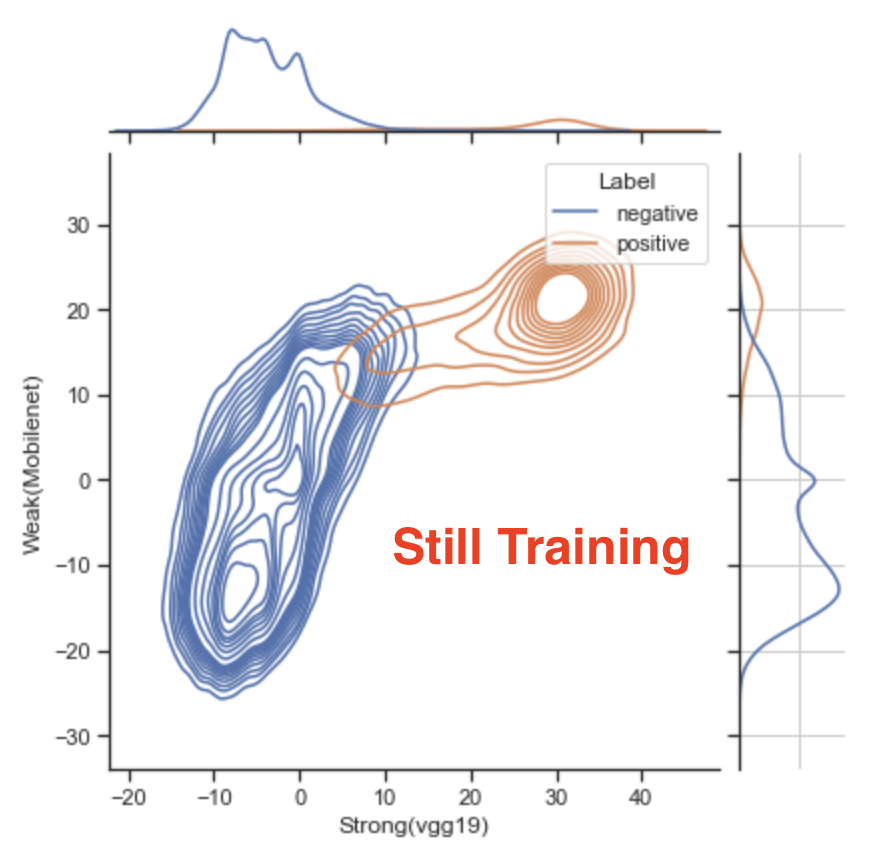
\includegraphics[width=2.5in]{figs/mobilenet_vgg_kde10_rsp.png}}
    \subfigure[Ensemble Size=100, Random Start]{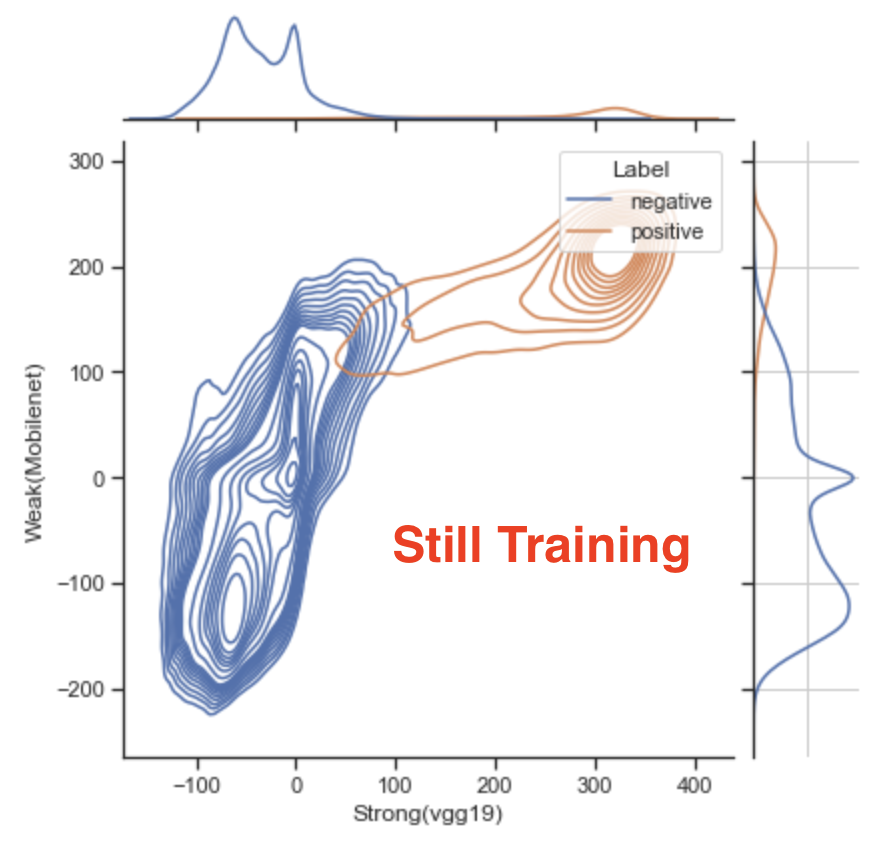
\includegraphics[width=2.5in]{figs/mobilenet_vgg_kde100_rsp.png}}
    \caption{\textbf{KDE Plot of Confidence of Strong and Weak Architectures}: The strong architecture is Vgg19, the weak architecture is MobileNet}
    \label{fig:kde_vgg_mobilenet}
\end{figure}


\subsection{Compare Human Results with Machine Results}
Following the framework shown in \ref{fig:struc}, we use the 3rd way in section \ref{sec:multi} and only set a single threshold for each architecture and allow prediction sets rather than only a single class as the output. Then for each image, each architecture will give a prediction set. We regard every class in the set as getting one vote from the architecture. Combine the sets by all the architectures, we get a collection. In this collection, each class among the 10 will get zero or one or multiple votes from the architectures. Based on the frequencies of each class's votes, we can measure how likely it is for each class to be chosen as a final prediction. With CIFAR10H, we can compare the results of human labeler and our machine predictors. Figure \ref{fig:example_prob} illustrates some examples that human and machine have the same confusion.

\begin{figure}[H]
    \centering
    \subfigure[]{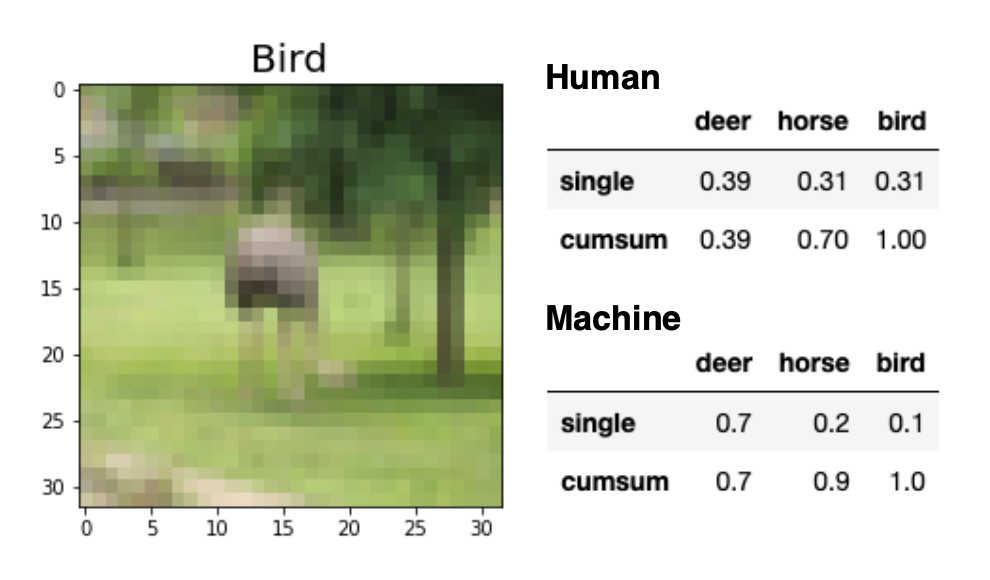
\includegraphics[scale=0.4]{figs/human_machine_agree_1.png}}
    \subfigure[]{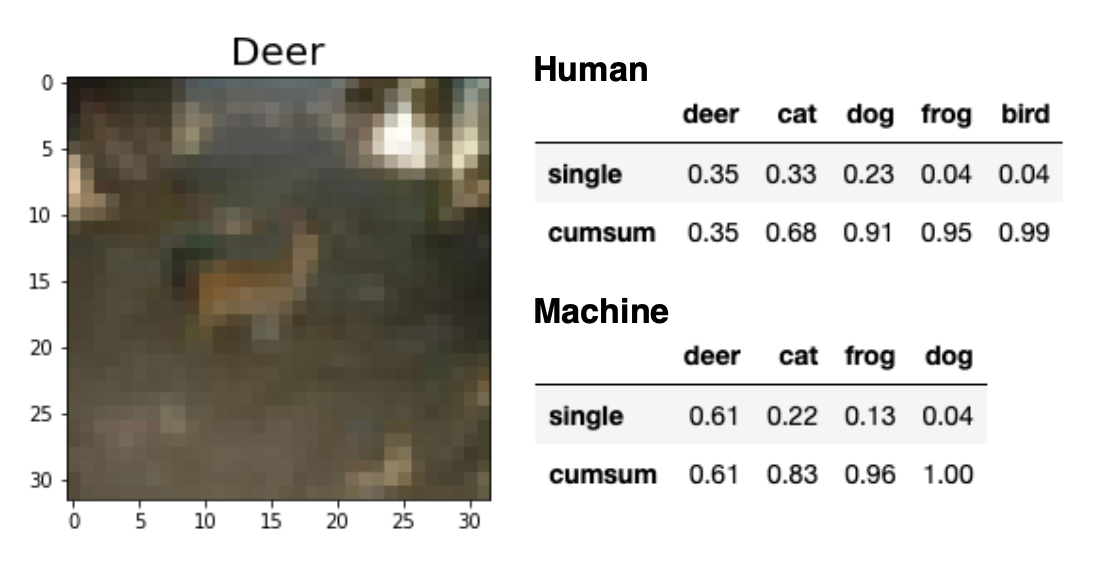
\includegraphics[scale=0.4]{figs/human_machine_agree_2.png}}
    \quad 
    \subfigure[]{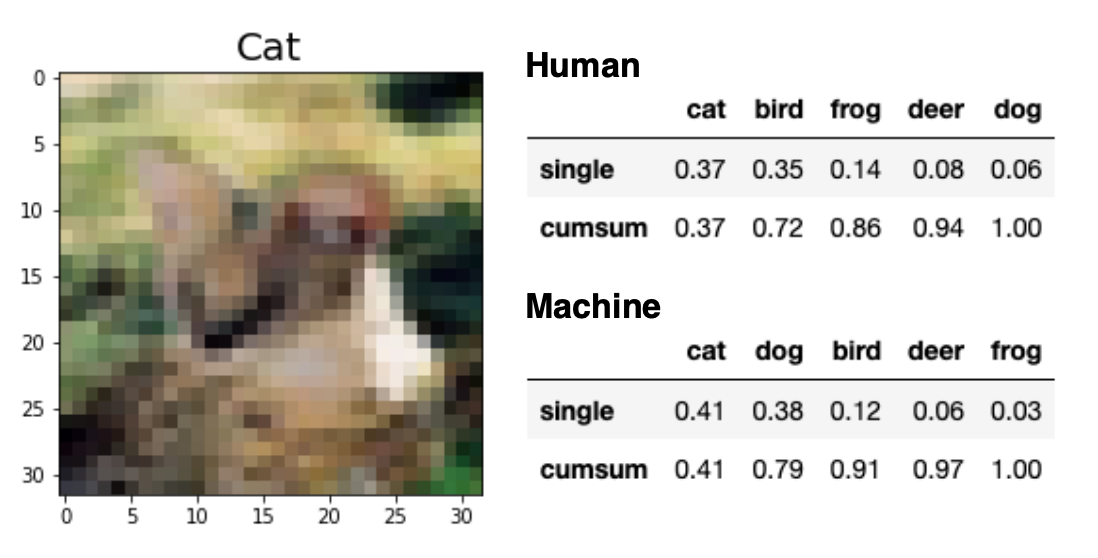
\includegraphics[scale=0.4]{figs/human_machine_agree_3.png}}
    \subfigure[]{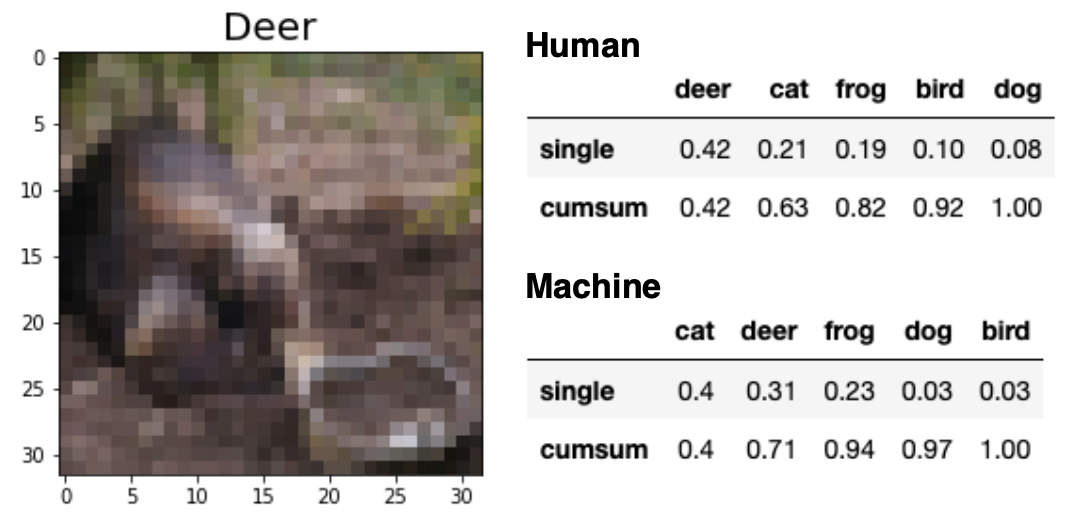
\includegraphics[scale=0.4]{figs/human_machine_agree_4.png}}
    \caption{\textbf{Examples That Human and Machine have the Same Confusion}: The tables shows the frequencies of votes of human labeler and machine predictors. The rows with index 'single' are the frequencies for each single class, the unshown classes all have zero frequencies. The rows with index 'cumsum' are the culmulative sum of the above row.}
    \label{fig:example_prob}
\end{figure}

For each image, we can use entropy of the frequency distribution by human/machine to measure how confusing it is for human/machine. We can use L1 distance between the frequency distributions by human and machine to measure their difference. We can denote each image as a point in the $\left[X,Y\right]$ plane where the $X$ axis is the machine entropy, and the $Y$ axis is the L1 distance between human and machine. A density plot is shown in Figure \ref{l1entropyscatter}

\begin{figure}[H]
    \centering
    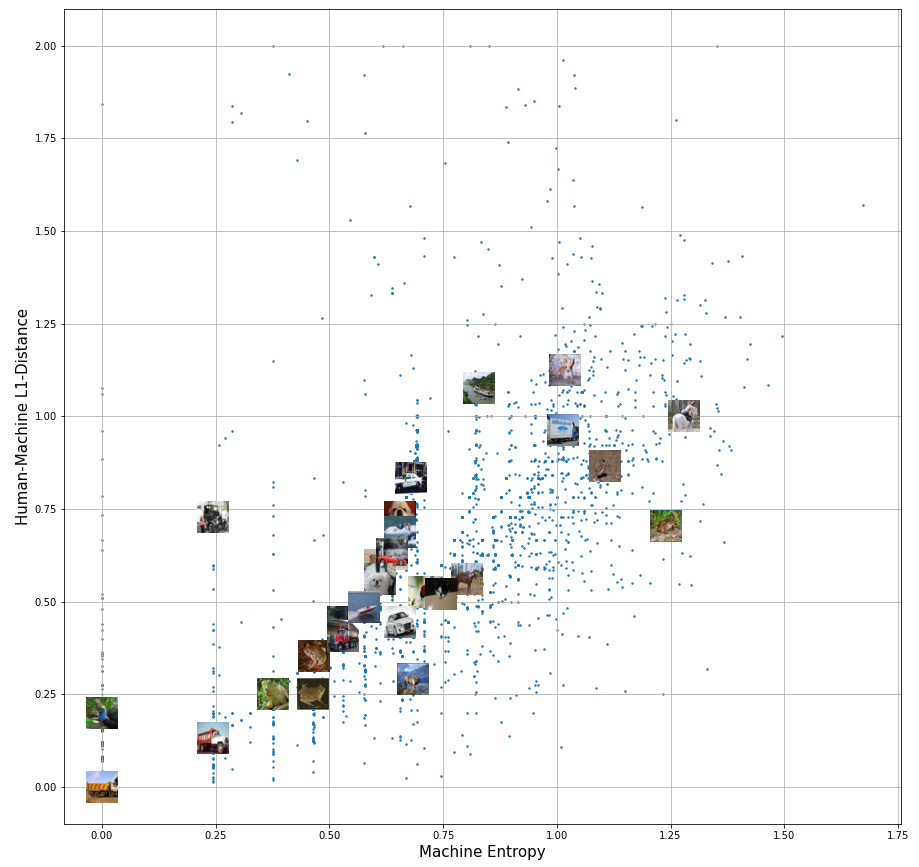
\includegraphics[scale=0.5]{figs/l1_entropy_scatter.png}
    \label{l1entropyscatter}
    \caption{\textbf{Entropy-L1 Scatter Plot}}
\end{figure}

\begin{figure}[H]
    \centering
    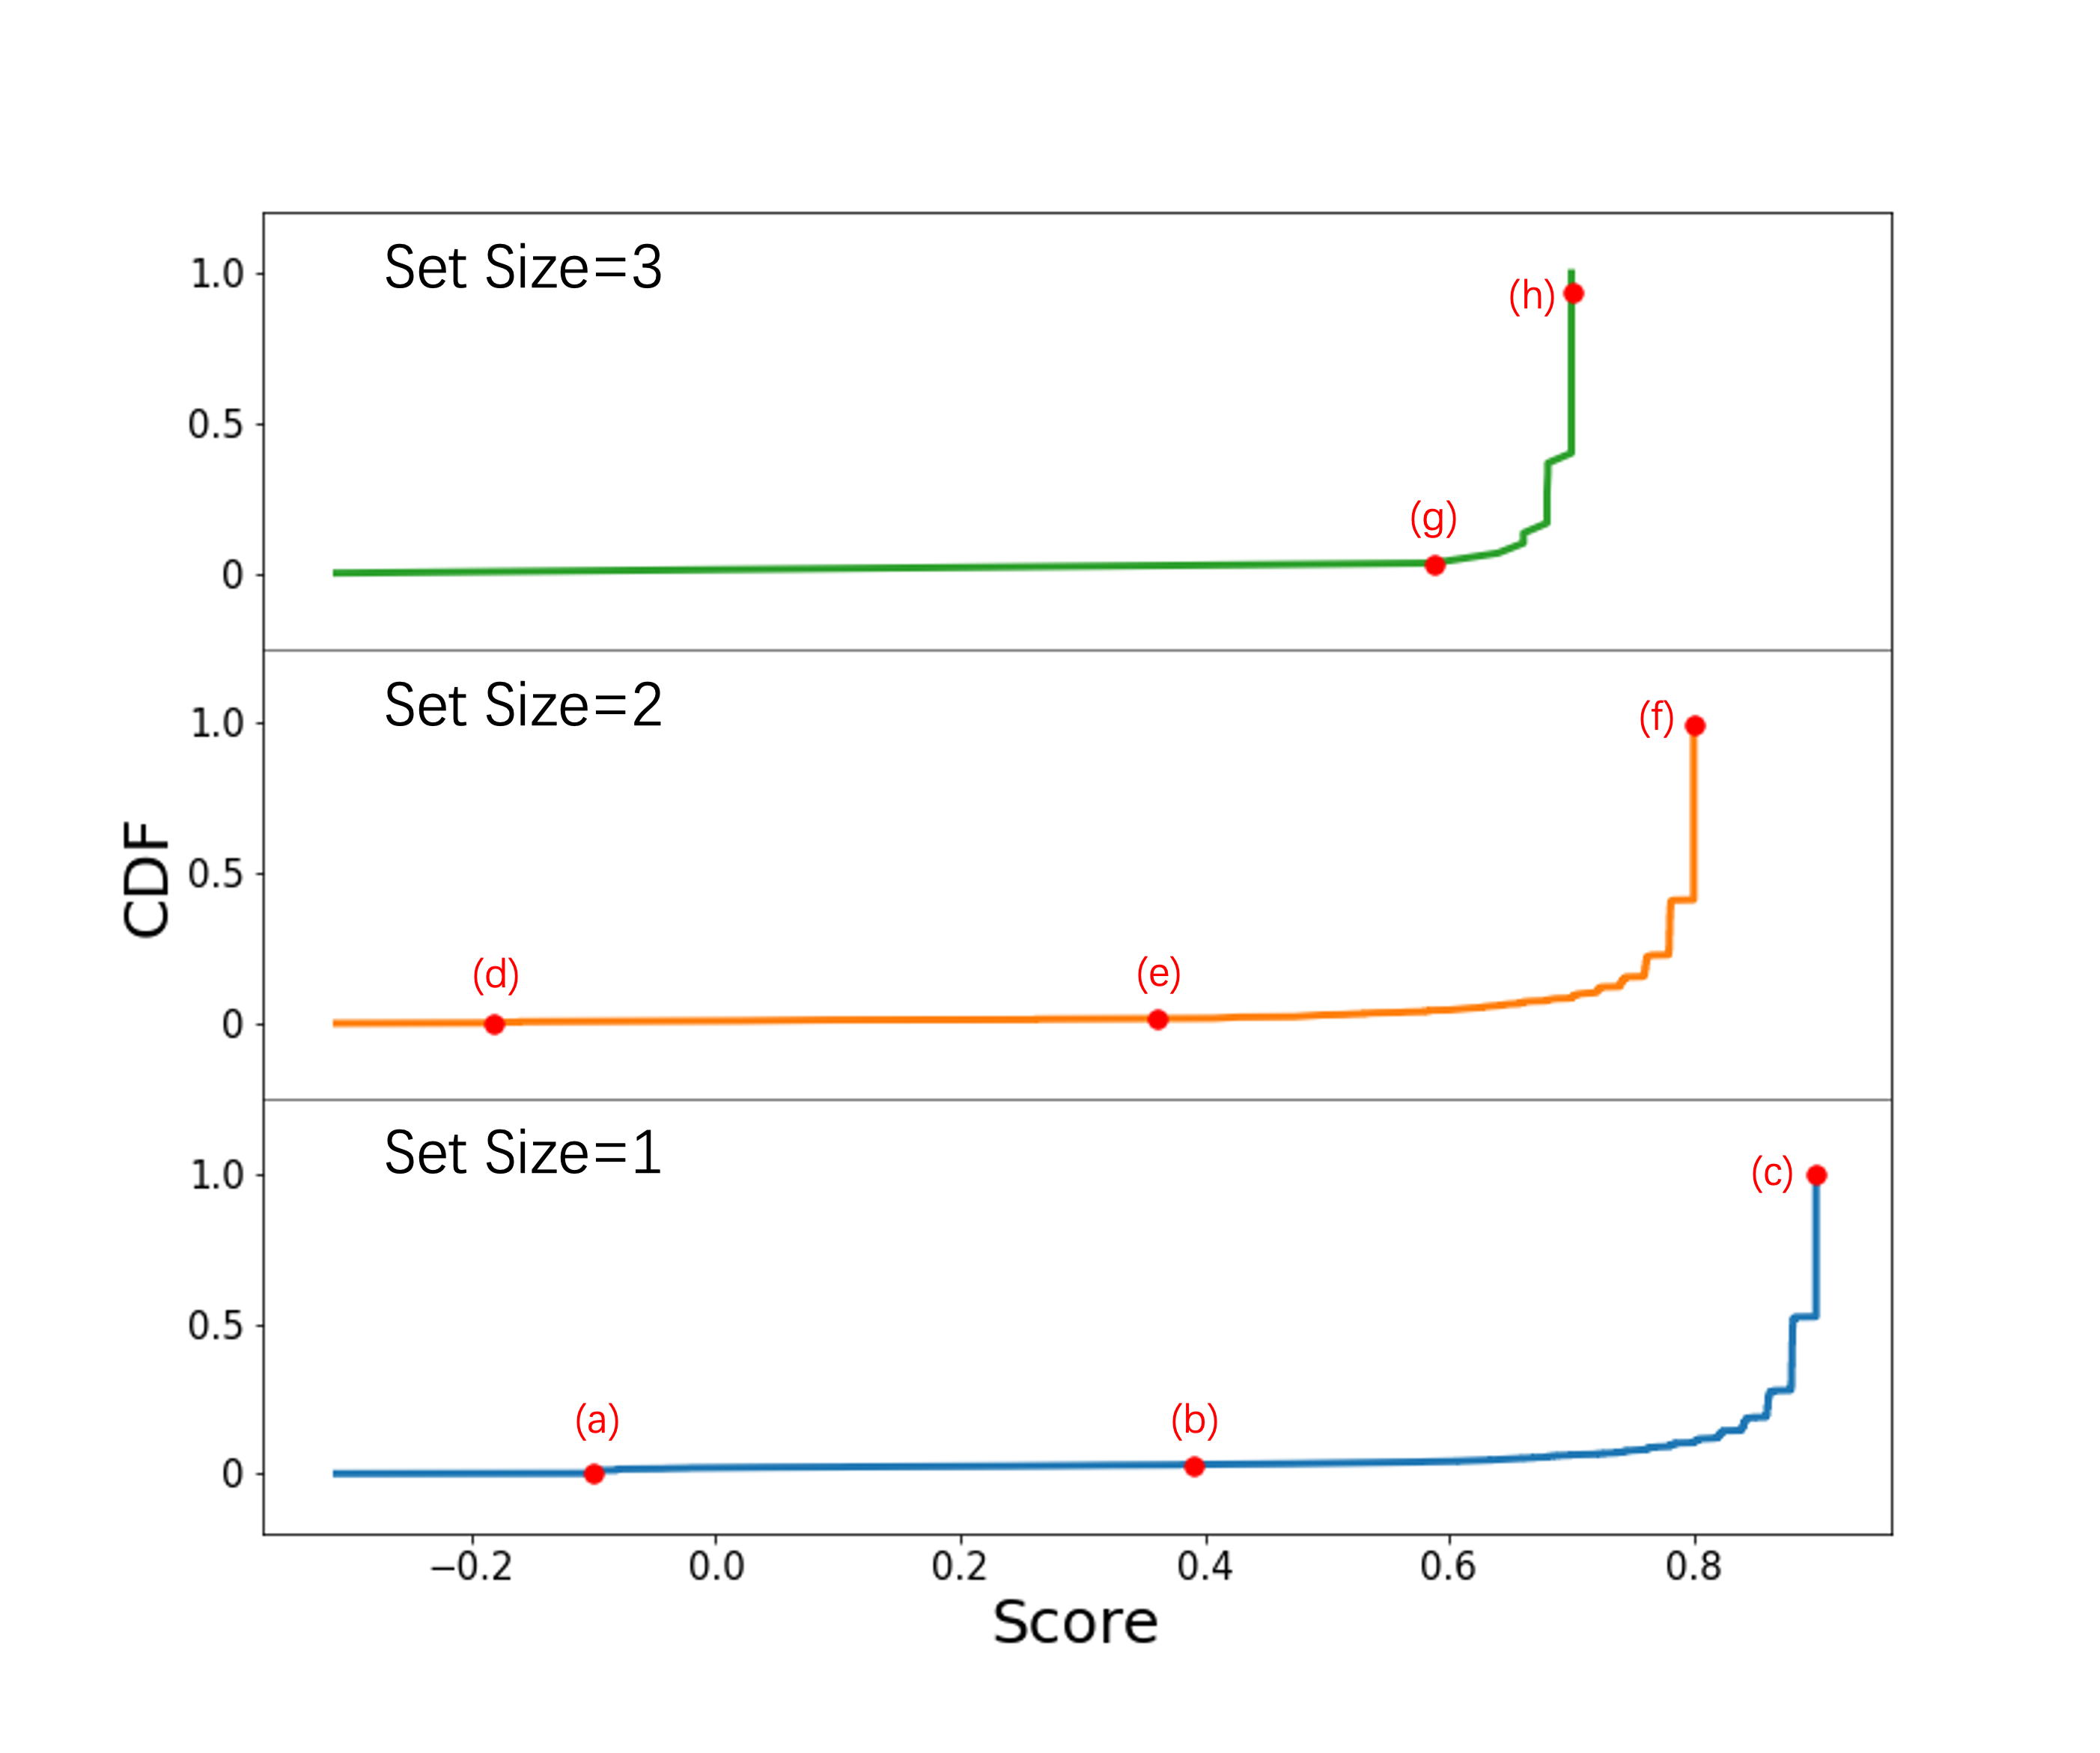
\includegraphics[scale=0.8]{figs/cdf_score_full.png}
    \label{cdf_score}
    \caption{\textbf{CDF of The Score for Different Set Sizes}}
\end{figure}


\begin{figure}[H]
    \centering

    \subfigure[]{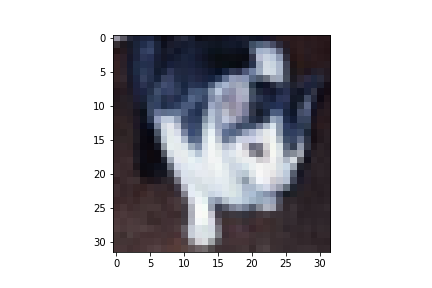
\includegraphics[scale=0.4]{figs/new_comb_fig/1_3594.png} \label{subfig:a}}
    \hspace{-28mm}
    \subfigure[]{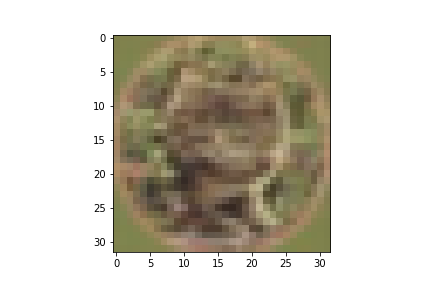
\includegraphics[scale=0.4]{figs/new_comb_fig/1_5511.png}}
    \hspace{-28mm}
    \subfigure[]{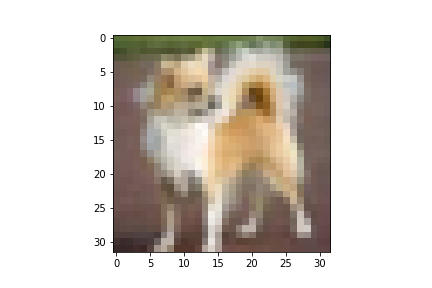
\includegraphics[scale=0.4]{figs/new_comb_fig/1_5035.png}}
    \hspace{-28mm}
    \subfigure[]{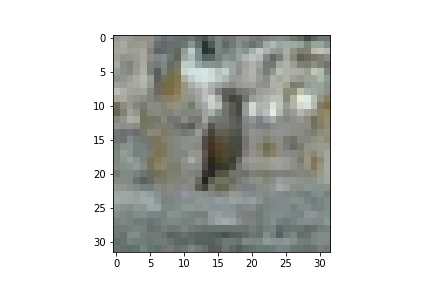
\includegraphics[scale=0.4]{figs/new_comb_fig/2_2270.png}}

    \subfigure[]{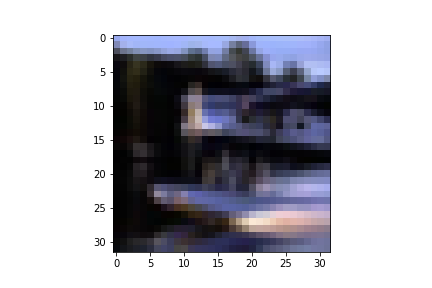
\includegraphics[scale=0.4]{figs/new_comb_fig/2_3211.png}}
    \hspace{-28mm}
    \subfigure[]{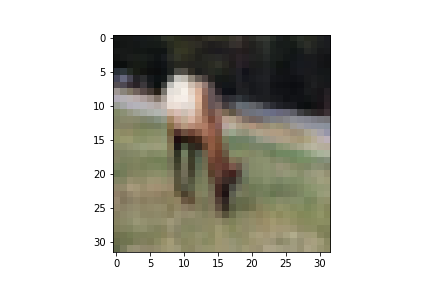
\includegraphics[scale=0.4]{figs/new_comb_fig/2_3962.png}}
    \hspace{-28mm}
    \subfigure[]{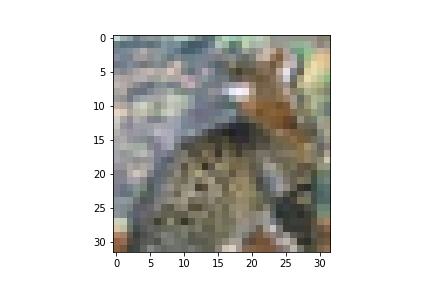
\includegraphics[scale=0.4]{figs/new_comb_fig/3_9497.png}}
    \hspace{-28mm}
    \subfigure[]{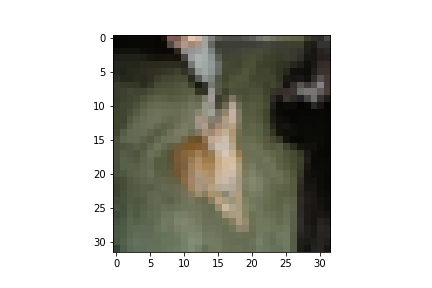
\includegraphics[scale=0.4]{figs/new_comb_fig/3_470.png}}
    \caption{\textbf{Examples of Human and Machine Classification} (a)\textbf{Human}: Cat(1.0). \textbf{Machine}: Dog. (b)\textbf{Human}: Frog(0.49), Cat(0.47), Bird(0.04). \textbf{Machine}: Frog. (c)\textbf{Human}: Dog(1.0). \textbf{Machine}: Dog. (d)\textbf{Human}: Bird(0.92), Ship(0.02), Frog(0.02), Dog(0.02), Cat(0.02). \textbf{Machine}: Cat, Dear. (e)\textbf{Human}: Airplane(0.56), Ship(0.44). \textbf{Machine}: Truck, Airplane. (f)\textbf{Human}: Deer(0.6), Horse(0.4). \textbf{Machine}: Deer, Horse. (g)\textbf{Human}: Cat(0.72), Frog(0.09), Deer(0.09), Bird(0.08), Airplane(0.02). \textbf{Machine}: Cat, Frog, Bird. (h)\textbf{Human}: Cat(0.65), Dog(0.21), Deer(0.14). \textbf{Machine}: Dog, Deer, Cat} 
    \label{fig:human_machine_example}
\end{figure}



\subsection{Example: Weak-Strong Flow}
To see how the above finds can be applied, we establish a weak-strong flow where we consturct an ensemble with a weak yet fast architecture and another ensemble with a strong yet slow architecture. For each coming image, the weak ensemble labels $+$, $-$, or $0$ for each class using the 3rd way in section \ref{sec:multi} with two thresholds, where $+$ represents being confident of belonging to this class, $-$ for confident of not belonging to this class, or $0$ for "I don't know" . If there is only one class with the label $+$, then this class will be the final result. Otherwise we call the strong the strong ensemble and make a prediction with the 1st way in section \ref{sec:multi}. 

The accuracy of this weak-strong flow is 0000. To compare, the accuracy for purly running an easy ensemble with the 1st way in section \ref{sec:multi} is 00000. The accuracy of running the strong ensemble only is 0000000

Table \ref{WSFlow} and \ref{strong_only} show the running time of the weak-strong flow and only running the strong ensemble.


\begin{table}
    \centering
    \begin{tabular}{crrrrr}
        \toprule
        {} Batch Size &  Weak Run &  Weak T-Test &  Strong Run &  Strong T-Test &  Weak-Strong Flow Total \\
        % Batch Size &           &              &             &                &                         \\
        \midrule
        16         &   0.54016 &      0.04063 &     3.38590 &        0.03598 &                 4.00267 \\
        64         &   0.32618 &      0.01138 &     2.32941 &        0.00957 &                 2.67653 \\
        256        &   0.42272 &      0.00420 &     2.83185 &        0.00308 &                 3.26185 \\
        1024       &   0.33215 &      0.00329 &     2.68724 &        0.00153 &                 3.02421 \\
        \bottomrule
    \end{tabular}
\label{WSFlow}
\caption{\textbf{Running Time of Weak-Strong Flow}: The weak model is MobileNet, the strong model is DPN92, the ensemble size for both architectures are 10. Batch Size indicates how how many images are processed parallelly by the weak-strong flow. The unit for all values is ms.}
\end{table}

\begin{table}
    \centering
    \begin{tabular}{crrr}
        \toprule
        {} Batch Size &  Strong Only Run &  Strong Only T-Test &  Strong Only Total \\
        % Batch Size &                  &                     &                    \\
        \midrule
        16         &          5.93767 &             0.03345 &            5.97112 \\
        64         &          4.93924 &             0.00943 &            4.94867 \\
        256        &          5.70755 &             0.00375 &            5.71130 \\
        1024       &          7.01784 &             0.00224 &            7.02008 \\
        \bottomrule
        \end{tabular}
\label{strong_only}
\caption{\textbf{Running Time of the Strong Ensemble Only}: The strong model is DPN92, the ensemble size is 10. Batch Size indicates how how many images are processed parallelly. The unit for all values is ms}
\end{table}

\bibliographystyle{plain}
\bibliography{refs.bib}

\end{document}

%%% Local Variables:
%%% mode: latex
%%% TeX-master: t
%%% End:
